\documentclass{article}
\usepackage[utf8]{inputenc}
% important for graphicx
\usepackage{graphicx}
\graphicspath{{img/}{src/}}
\usepackage{float}
\usepackage{hyperref}
\usepackage{enumitem}
\usepackage{algorithm}
\usepackage{subcaption}
\usepackage[mathscr]{euscript}
\usepackage[detect-all]{siunitx}
\usepackage[noend]{algpseudocode}
% background color for definitions
\usepackage[most]{tcolorbox}
\tcbset{
    frame code={}
    center title,
    left=0pt,
    right=0pt,
    top=0pt,
    bottom=0pt,
    colback=blue!6!white,
    colframe=white,
    width=\dimexpr\textwidth\relax,
    enlarge left by=0mm,
    boxsep=10pt,
    arc=0pt,outer arc=0pt,
}

\newenvironment{changemargin}[2]{%
\begin{list}{}{%
\setlength{\topsep}{0pt}%
\setlength{\leftmargin}{#1}%
\setlength{\rightmargin}{#2}%
\setlength{\listparindent}{\parindent}%
\setlength{\itemindent}{\parindent}%
\setlength{\parsep}{\parskip}%
}%
\item[]}{\end{list}}

\usepackage{listings}
\usepackage{xcolor}

%New colors defined below
\definecolor{codegreen}{rgb}{0,0.6,0}
\definecolor{codegray}{rgb}{0.5,0.5,0.5}
\definecolor{codepurple}{rgb}{0.58,0,0.82}
\definecolor{backcolour}{rgb}{0.95,0.95,0.92}

%Code listing style named "mystyle"
\lstdefinestyle{mystyle}{
  backgroundcolor=\color{backcolour},   commentstyle=\color{codegreen},
  keywordstyle=\color{magenta},
  numberstyle=\tiny\color{codegray},
  stringstyle=\color{codepurple},
  basicstyle=\ttfamily\footnotesize,
  breakatwhitespace=false,         
  breaklines=true,                 
  captionpos=b,                    
  keepspaces=true,                 
  numbers=left,                    
  numbersep=5pt,                  
  showspaces=false,                
  showstringspaces=false,
  showtabs=false,                  
  tabsize=2
}

%"mystyle" code listing set
\lstset{style=mystyle}

\title{Code Listing}
\date{ }

\begin{document}

\title{Image Processing III\\
Mutual Information}
\author{Aadil Anil Kumar \\
Otmane Sabir
}
\date{26/4/2020}
\maketitle
\vspace{10mm}
\begin{center}
\section*{Introduction}
\large
The third homework assignment required us to implement the similarity metric algorithm "mutual information" while following certain guidelines which could be summarized to the following list: 
\vspace{7mm}
\begin{enumerate}
    \item Implement the algorithm.
    \item Choose 3 images from the internet and separate the green and red channels as two separate gray scale images each. Crop the green channel by cutting 20 pixels from the left and right sides, respectively - resulting in a cropped green channel image with 40 pixels smaller than the red channel image. Then virtually move the red channel images in x-direction over the corresponding green channel image in 41 steps from the left to right, and compute the mutual information of the overlapping regions for every step.
    \item Plot the mutual information as a function of the x-position of the red channel image for all three chosen red/green image pairs.
\end{enumerate}


\end{center}
\newpage

\tableofcontents

\newpage

\section{Mutual Information}
\vspace{2mm}
\begin{flushleft}
Mutual information is a quantity that measures a relationship between two random variables that are sampled simultaneously. In particular, it measures how much information is communicated, on average, in one random variable about another. For example, suppose X represents the roll of a fair 6-sided die, and Y represents whether the roll is even (0 if even, 1 if odd). Clearly, the value of Y tells us something about the value of X and vice versa. That is, these variables share mutual information. \cite{entropy&mi}
\end{flushleft}
\vspace{2mm}
\begin{figure}[ht]
    \centering
    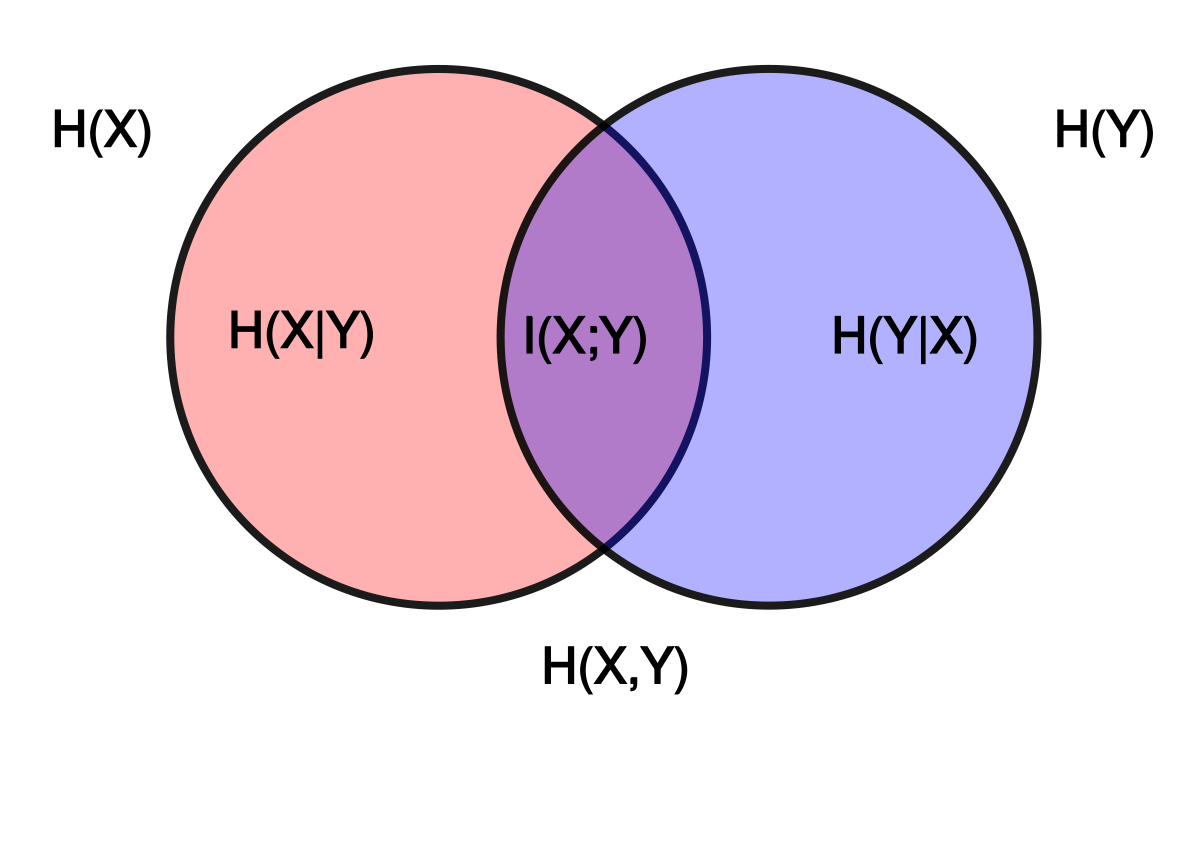
\includegraphics[width=\linewidth]{mutual information.png}
    \caption{Mutual Information Visualization}
    \label{fig:watershed_visualization}
\end{figure}

\subsection{Formal Definition}
\begin{flushleft}
\vspace{2mm }
\begin{tcolorbox}
\textsc{Definition:}\cite{wiki}\cite{quantiki}\newline\newline
The formal definition of the mutual information of two random variables $X$ and $Y$, whose joint distribution is defined by $P(X, Y)$ is given by
\vspace{4mm}
\begin{center}
\[
I(X;Y) = \sum_{x \in X}^{}\sum_{y \in Y}^{} P(x, y)\log \frac{P(x, y)}{P(x)P(y)}
\]
\end{center}
Such that, $P(X)$ and $P(Y)$ are the \textit{marginal distributions} of $X$ and $Y$ obtained through the marginalization process which can be defined as : 
\begin{center}
\[
p_X(x_i) = \sum_{j}p(x_i, y_i)
\]

\[
p_Y(y_j) = \sum_{i}p(x_i, y_i) 
\]
\end{center}
\end{tcolorbox}
\end{flushleft}

\section{Shannon Entropy \& Mutual Information}
\vspace{2mm}
\begin{flushleft}
In our implementation, we rely on calculating the shannon entropy in order to estimate the mutual information. Intuitively, some may ask what is entropy? 
\end{flushleft}
The entropy is the expected value of the self-information, the self-information quantifies the level of information or surprise associated with one particular outcome or event of a random variable, whereas the entropy quantifies how "informative" or "surprising" the entire random variable is, averaged on all its possible outcomes.

\subsection{Formal Definition : Shannon Entropy}
\label{marker}
\vspace{2mm}
\begin{flushleft}
\vspace{2mm }
\begin{tcolorbox}
\textsc{Definition:}\cite{wiki-shannon}\newline\newline
The formal definition of the entropy of a discrete random variable $X$ with possible values $\{x_1, ... ,x_n\}$ and probability mass function $P(X)$ is
\vspace{4mm}
\begin{center}
\[
H(X) = - \sum{P(x_i)\log_b P(x_i)}
\]
\end{center}
\vspace{4mm}
where $b$ is the base of the logarithm used. Common values of b are 2, Euler's number $e$, and 10. In the case of $P(x_i) = 0$ for some $i$, the value of the corresponding summand $0\log_b (0)$ is taken to be 0.
\end{tcolorbox}
\end{flushleft}

\subsection{Formal definition : Mutual Information}
\label{marker2}
\vspace{2mm}
\begin{flushleft}
\vspace{2mm}
\begin{tcolorbox}
\textsc{Definition:}\cite{quantiki}\newline\newline
If we consider pairs of discrete random variables (X,Y), then formally, the mutual information can be defined as :
\begin{center}
\[
I(X : Y) = H(X) + H(Y) - H(XY)
\]
\end{center}
\vspace{2mm}
with $H(X)$, $H(Y)$ the Shannon entropy of $X$ an $Y$, and $H(XY)$ the Shannon entropy of the pair $(X, Y)$. 
\end{tcolorbox}
\end{flushleft}

\section{Implementation}
\vspace{2mm}
\begin{flushleft}
We decided to implement our algorithm in python for ease of implementation and the support provided from preexisting libraries. We first started by implementing a simple entropy computation method, then by interpreting the image signals from the image to match our entropy function and then applying the formula from the previous definition.

Before we start implementing, this is a list of all libraries and styles used in order to calculate, convert and plot our results.
\end{flushleft}
\begin{lstlisting}[language=Python]
import numpy as np
import matplotlib.pyplot as plt
import seaborn as sns
from scipy.stats import entropy as scipy_entropy
from PIL import Image
plt.style.use('seaborn')
\end{lstlisting}

\subsection{Entropy function :}
\vspace{2mm}
\begin{flushleft}
This is a simple implementation of the entropy function. Given the input parameter $X$ which in our case is a random variable, we get the entropy of the random variable. In subsection \textbf{\ref{marker}} we introduced a formal definition of this calculation.
\end{flushleft}
\begin{lstlisting}[language=Python, caption=Entropy Calculator]
def entropyCalc(X):
    uniq = set(X)
    P = [np.mean(X == x) for x in uniq]
    return sum(-p * np.log2(p) for p in P)

\end{lstlisting}

\subsection{Converting the image}
\vspace{2mm}
\begin{flushleft}
In order for our entropy function to properly compute these values we need to convert the image from the matrices we receive to appropriate signals. We do this by using the numpy histogram functions in the case of the join histogram.
\end{flushleft}
\begin{lstlisting}[language=Python, caption=1D Signal]
def convert1DSignal(x, nBins):
    return np.histogram(np.asarray(x).flatten(), bins=nBins)[0]
\end{lstlisting}

\begin{lstlisting}[language=Python, caption=2D Signal (Joint Histogram)]
def convert2DSignal(x, y, nBins):
    hist = np.histogram2d(np.asarray(x).flatten(), np.asarray(y).flatten(), bins=nBins)
    return np.asarray(Image.fromarray(hist[0], 'RGB')).flatten()
\end{lstlisting}

\subsection{Mutual Information}
\begin{flushleft}
We now have all the required tools to calculate our mutual information estimation. The mutual information function will be very simple and will follow our definition in the subsection \textbf{\ref{marker2}}.
\end{flushleft}

\begin{lstlisting}[language=Python, caption=Mutual Information]
def mutualInformation(x, y, nBins):
    HX = entropyCalc(convert1DSignal(x, nBins))
    HY = entropyCalc(convert1DSignal(y, nBins))
    HXY = entropyCalc(convert2DSignal(x, y, nBins))
    return HX + HY - HXY
\end{lstlisting}

\section{Experiments \& Results}
\vspace{2mm}
\begin{flushleft}
The experiments we were asked to conduct were an intuitive way of visualizing how mutual information exactly works. We were asked to choose 3 images from the internet and separate the green and red channels as two separate gray scale images each. Crop the green channel by cutting 20 pixels from the left and right sides, respectively - resulting in a cropped green channel image with 40 pixels smaller than the red channel image. Then virtually move the red channel images in x-direction over the corresponding green channel image in 41 steps from the left to right, and compute the mutual information of the overlapping regions for every step and then finally plot the mutual information as a function of the x-position of the red channel image for all three chosen red/green image pairs. \newline

Before we proceed, we want to clarify the difference between bin size and number of bins. Given that x is the bin size we want, that y is the number of bins and that the image is a gray scale image - meaning the maximum number of bins is 256 - then $y = 256/x$ or $x = 256/y$ which will explain the nature of the varying number of bins plots (See figures \ref{fig:puffin_binSize}, \ref{fig:balloon_binSize} \& \ref{fig:flower_binSize}.)

\subsection{Test function implementation}
\vspace{2mm}
\begin{flushleft}
In order to achieve this we had to create a function which would trim the given image from the sides and create all other possible crops since our mutual information can't take signals of different sizes as it will be comparing a given value to nothing which would always return an error; therefore, our approach was to create a symmetrically cropped image from as the top image and create a list of all possible cropped images starting from 40 pixels to right to 40 to the left.
\end{flushleft}

\begin{lstlisting}[language=Python, caption=Mutual Information]
def cropImage(img):
    r, g, b = splitImage(img)
    w, h = img.size
    top = r.crop((20, 0, w-20, h))
    return top, [g.crop((40-x, 0, w-x, h)) for x in range(40, -1, -1)]
\end{lstlisting}
\end{flushleft}

% ----------------------------------------- PUFFIN EXPERIMENT  -----------------------------------------

\subsection{Puffin Experiment}
\vspace{2mm}

\begin{flushleft}
For the first experiment, we decided to use a 800X800 puffin image (See Figure \ref{fig:puffin_original}). We then ran our test functions with different bin sizes and with image translations.
\end{flushleft}

\begin{figure}[H]
    \centering
    \includegraphics[width=\linewidth]{experiments/puffin/RGB1-Puffin.png}
    \caption{Original Puffin Image \& Splits.}
    \label{fig:puffin_original}
\end{figure}

\begin{flushleft}
The results we got were as expected (see Figure \ref{fig:puffin_translations}). The mutual information value peaks when the the image translations is at 20 as it has reached the optimal combination of the red and green channels since both images are now symmetrically cropped (20 pixels from left and 20 from the right).
\end{flushleft}
\begin{figure}[H]
    \centering
    \includegraphics[width=\linewidth]{experiments/puffin/puffin-translations.png}
    \caption{Translation Test with MI }
    \label{fig:puffin_translations}
\end{figure}

\begin{flushleft}
The results we got were as expected (see Figure \ref{fig:puffin_binSize}). The mutual information approximation drops as we increase the bin size as it becomes less and less precise the higher our bin size gets until it completely flattens out and finds no mutual information. 
\end{flushleft}

\begin{figure}[H]
    \centering
    \includegraphics[width=\linewidth]{experiments/puffin/puffin-binSize.png}
    \caption{Bin Size Change - Puffin}
    \label{fig:puffin_binSize}
\end{figure}

% ----------------------------------------- BALLOON EXPERIMENT  -----------------------------------------

\subsection{Balloon Experiment}
\vspace{2mm}

\begin{flushleft}
For the second experiment, we decided to use a 1024X694 balloon image (See Figure \ref{fig:balloon_original}). We then ran our test functions with different bin sizes and with image translations.
\end{flushleft}

\begin{figure}[H]
    \centering
    \includegraphics[width=12cm]{experiments/balloon/RGB1-Balloon.png}
    \caption{Original Balloon Image \& Splits.}
    \label{fig:balloon_original}
\end{figure}

\begin{flushleft}
While the results were not as steady as the previous experiment but these also allow us to interpret the function from a different point a view and open a new level of understanding. As we can see in the original image splits (Figure \ref{fig:balloon_original}). The resulting gray scale images are quite different from each other allowing more room for fluctuation and less mutual information which directly translates to the result we got in Figure \ref{fig:balloon_translations} since we can't exactly predict how the red and green channels look like during the translation but it remains correct that the mutual information peaks when it reaches the symmetric crop.
\end{flushleft}

\begin{figure}[H]
    \centering
    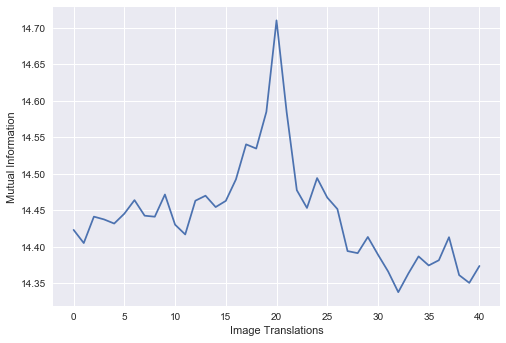
\includegraphics[width=\linewidth]{experiments/balloon/balloon-translations.png}
    \caption{Translation Test with MI - Balloon}
    \label{fig:balloon_translations}
\end{figure}

\begin{flushleft}
We can see that the results are similar to the previous one. As the number of bins increases, the mutual information increases since we, again, have more "information" than with previous images. It's also important to mention that the MI increases because the images are relatively similar and that only few gray scale values differ which explain why for this scenario the MI increase the higher the number of bins.
\end{flushleft}

\begin{figure}[H]
    \centering
    \includegraphics[width=\linewidth]{experiments/balloon/balloon-binSize.png}
    \caption{Bin Size Change - Balloon}
    \label{fig:balloon_binSize}
\end{figure}

% ----------------------------------------- FLOWER EXPERIMENT  -----------------------------------------

\subsection{Flower Experiment}
\vspace{2mm}

\begin{flushleft}
For experiment 3 we used a 256x256 flower image (See Figure \ref{fig:puffin_original} and ran the same tests as in the two past experiments.
\end{flushleft}

\begin{figure}[H]
    \centering
    \includegraphics[width=12cm]{experiments/flower/RGB1-Flower.png}
    \caption{Original Flower Image \& Splits.}
    \label{fig:flower_original}
\end{figure}

\begin{flushleft}
The results showed a lot more fluctuation this time but kept the peak at the same place (Figure \ref{fig:flower_translations}. We can first explain these by the big difference in the green and red gray scale images (See Figure \ref{fig:flower_original}. 
Another reason the fluctuations are higher could be the image resolutions since each pixel shift has a lot more "weight". For example, shifting by one column of pixels in a 800X800 image means we're changing around 0.125\% of the image while shifting by one column in a 256X256 image means we're changing 0.39\% of the image which gives the shift more importance as the image is smaller.
\end{flushleft}

\begin{figure}[H]
    \centering
    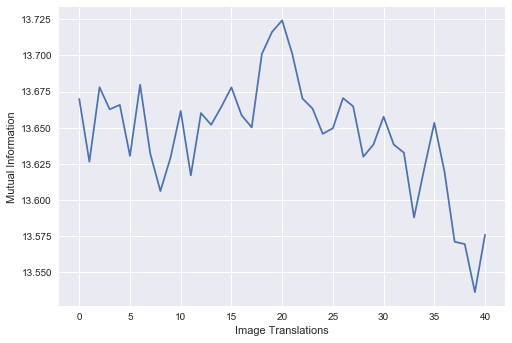
\includegraphics[width=\linewidth]{experiments/flower/flower-translations.png}
    \caption{Translation Test with MI - Flower}
    \label{fig:flower_translations}
\end{figure}

\begin{flushleft}
The results were again similar to both previous experiments which confirm our explanation.
\end{flushleft}

\begin{figure}[H]
    \centering
    \includegraphics[width=\linewidth]{experiments/flower/flower-binSize.png}
    \caption{Bin Size Change - Flower}
    \label{fig:flower_binSize}
\end{figure}


\newpage

\begin{thebibliography}{9}
\label{sec:hello}

\bibitem{entropy&mi}
Entropy and Mutual Information: \newline
AS Kornillov
\\\texttt{https://people.cs.umass.edu/~elm/Teaching/Docs/mutInf.pdf}

\bibitem{wiki}
Mutual Information: \newline
Wikipedia 
\\
\texttt{https://en.wikipedia.org/wiki/Mutual_information}

\bibitem{quantiki}
Mutual Information : \newline
Quantiki :
\\
\texttt{https://www.quantiki.org/wiki/mutual-information}

\bibitem{wiki-shannon}
Entropy (Information Theory) : \newline
Wikipedia :
\\
\texttt{https://en.wikipedia.org/wiki/Entropy_(information_theory)}

\end{thebibliography}

\end{document}
